% This must be in the first 5 lines to tell arXiv to use pdfLaTeX, which is strongly recommended.
\pdfoutput=1
% In particular, the hyperref package requires pdfLaTeX in order to break URLs across lines.

\documentclass[11pt]{article}

% Remove the "review" option to generate the final version.
% \usepackage[review]{acl}
\usepackage{acl}

% Standard package includes
\usepackage{times}
\usepackage{latexsym}
\usepackage{booktabs}
\usepackage{graphicx}
\usepackage[normalem]{ulem}
\useunder{\uline}{\ul}{}

% For proper rendering and hyphenation of words containing Latin characters (including in bib files)
\usepackage[T1]{fontenc}
% For Vietnamese characters
% \usepackage[T5]{fontenc}
% See https://www.latex-project.org/help/documentation/encguide.pdf for other character sets

% This assumes your files are encoded as UTF8
\usepackage[utf8]{inputenc}

% This is not strictly necessary, and may be commented out,
% but it will improve the layout of the manuscript,
% and will typically save some space.
\usepackage{microtype}

% If the title and author information does not fit in the area allocated, uncomment the following
%
\setlength\titlebox{5cm}
%
% and set <dim> to something 5cm or larger.

\title{A Toxicity Detection Dataset with r/WallStreetBet Comments}


\author{Amelia Chu, Yunseok Jang, Graham Murphy \and Yoon Tae Park \\
 Center for Data Science \\ New York University \\ 60 5th Avenue, New York, NY \\
  \texttt{\{ameliachu, yj2369, gm2858, yp2201\}@nyu.edu} \\}
  
% Author information can be set in various styles:
% For several authors from the same institution:
% \author{Author 1 \and ... \and Author n \\
%         Address line \\ ... \\ Address line}


\begin{document}
\maketitle

\begin{abstract}
Toxicity is a common pain point that is tasking on both contributors and moderators of online forums. Although there are existing toxicity classification datasets, many do not have high inter-rater reliability. In this project, we provide a new toxicity detection dataset using comments from r/WallStreetBets and toxicity attribute labels from \citet{Perspective2022}. This dataset was generated with an accompanying codebook and review process which allowed the labelers to achieve a higher inter-rater reliability. Therefore, consumers of our new dataset can have a better understanding of the resulting labels.

\end{abstract}

\section{Introduction \& Background}
Toxicity is a common pain point in online forums. It is tasking on contributors and can lead to users disengaging from conversations, attrition, or even impact the safety of the community \citep{vidgen2021, salminen2020}. It is also tasking on moderators, who often become overwhelmed and fatigued from viewing toxic comments \citep{almerekhi2020, vidgen2020}.  Therefore, to make social media platforms a more hospitable place, it is important to detect and remove toxic comments for the overall community wellbeing.  An example of a forum that suffers from this kind of toxicity is the subreddit WallStreetBets. Traditionally known and visited by few, in recent years r/WallStreetBets has drawn attention from mainstream media outlets as a premier example of a toxic forum \citep{harwell2021, hadly2021, mccabe2021}. 

Although there are existing text classification datasets with toxicity or malevolent attributes, these attributes can be hard to define, or it may be difficult to obtain a consensus \citep{davidson2017, salminen2018, salminen2019}. Likewise, interrater reliability can be low, as was the case with the CAD dataset \citep{vidgen2021}. In the GoEmotions dataset, although interrater reliability was high amongst positive emotions, items with negative emotion had larger disagreements \citep{demszky2020}.In other cases where interrater reliability is higher, such as in \citet{pavlick2019},  \citet{salminen2020}, and \citet{zhang2021}, more short-form text content was used (i.e. Twitter data). We believe there is an opportunity to introduce new data into the current toxic-sentiment classifier landscape to potentially expose shortcomings. Particularly, we hope to establish a dataset that is able to have a high interrater reliability, by ensuring our labelers have a common interpretation of the definitions for each of the toxic attribute labels in our dataset. To this end, we will be electing to not use crowdsourced labels. As found in \citet{vidgen2020}, though crowdsourcing labels can be an efficient way to collect labeled data, it is difficult to ensure all crowdworkers have the same interpretation of a task. 

In this project, we provide a new benchmark dataset\footnote{https://github.com/ameliachu/nlu-reddit-toxicity-dataset} using comments from r/WallStreetBets and toxicity attribute labels that is not well classified by using current SOTA models, and thereby enriching publicly available datasets for testing toxicity.



\section{Data}
\subsection{Data Collection}
To construct our dataset, we used pre-collected data from r/WallStreetBets. This pre-collected data contains 619, 646 comments from ``Daily Discussion Thread'' submissions from the end of January 2021 to April 2021. This time period coincides with when  r/WallStreetBets became popular and had a variety of moderating issues \citep{mcenery2021}. The daily discussion submissions were chosen because those threads were designed to attract all users, not just niche topics or community experts. 

Users are encouraged to interact and post quick questions, thus these submissions attracted users of varying experience and commitment to the r/WallStreetBets community \citep{wsb2022}. The data pipeline used to collect this data used PRAW (Python Reddit API Wrapper) and used tokens provided by Reddit to ensure alignment with Reddit's Terms of Service. 

From this pre-collected dataset, we randomly selected and assigned batches of 200 new comments and 60 previously rated comments for each of our 4 raters. As the dataset is overwhelmingly ``non-toxic'' (see Table~\ref{data-distribution}), this random batch assignment continued until we had approximately 500 comments with at least 1 toxic attribute. We labeled the data in batches so that raters could periodically check-in, discuss any ambiguity, raise concerns and revise the codebook as needed (See Section 2.2.1 for further detail). Of the 2,441 comments reviewed, 800 were selected for the final dataset. All examples with at least one toxic attribute (\emph{n}=483) were retained, some curated ``non-toxic'' examples (e.g. contains an identity mention, but not did not qualify as an attack) were included, and finally, 293 remaining ``non-toxic''  examples were randomly selected.  The final dataset has a distribution that skews more toward ``toxic'' examples than original dataset, as a differentiating feature of this dataset is the abundance of examples which may contain toxic attributes, but do not ultimately meet the definition of "toxicity" (as defined in Table~\ref{label-definitions}).


\subsection{Data Taxonomy \& Labeling Methodology}

The pre-collected data was reshaped so each comment selected for labeling included context (i.e. the preceding and following comment). Then, each comment was labeled by human raters (i.e. the authors of this paper) for the presence of 5 toxic attributes: toxicity, severe toxicity, identity attack, insult, profanity, threat. For each attribute, raters will assign a value 1 if they believe the comment matches the definition of a toxic attribute, or assign 0, if they do not believe the comment matches the definition (See Table Table~\ref{label-definitions} for a full list of definitions). Raters were asked to use the definitions provided by \citet{Perspective2022} and to evaluate each label independently. For example, even if a comment is determined to contain profanity, this does not mean it meets the definition of toxicity. Likewise, there appears to be low correlation between the toxic attributes Figure~\ref{heatmap-corr}. The highest correlation between attributes is between toxicity and insult (\emph{r}=0.63). Each human rater was instructed to consider the context if there was any uncertainty on whether a comment had a toxic attribute.

\subsubsection{Inter-rater Reliability}
Inter-rater reliability was evaluated through an initial assessment and will be routinely re-evaluated throughout the dataset generation period. 

\paragraph{Initial Assessment.}
The initial assessment generated by randomly sampling the pre-collected dataset, selecting examples that were likely to contain one or more toxic attributes, repeating the random sample process until 10 comments were selected. Before taking the assessment, raters, as a group, reviewed the toxic attribute definitions and practiced labeling those attributes on a separate set of 5 examples. Any ambiguity or clarifying questions raised would be discussed until a consensus is reached. When needed, a guideline would be recorded for the codebook \footnote{https://github.com/ameliachu/nlu-reddit-toxicity-dataset/blob/main/artifacts/codebook.md}.

After the group exercise, the raters performed the interrater assessment independently. Inter-rater reliability was assessed with Spearman's R. Overall, the raters achieved an initial reliability of 0.71, however there was low initial agreement on the toxicity label (\emph{r}=0.5) and no comments were identified with ``threat'' attribute as part of the initial assessment.


\paragraph{Routine evaluation methodology.}

To ensure and re-enforce consistency, raters received randomly-selected batches of 260 comments for evaluation, at a time. When all raters complete a batch, for a total of 1,040 comments, they convene to discuss any examples while those examples are relatively top-of-mind. If there are any examples they found ambiguous, they are encouraged to discuss with the group, and if needed, the codebook guidelines would then be updated to reflect new or changed criteria. The raters are free to return to their assigned examples to revise any labels to reflect the latest updates to the codebook. 

Additionally, this batch method enables us to routinely assess our interrater reliability. Aside from the initial batch, each subsequent batch contained 200 new examples and 60 randomly selected examples that have been already rated by another rater. These 60 examples are evaluated for inter-rater reliability and serve as a checkpoint to potentially help determine if we need to revise any labeling guidelines. Overall, the raters achieved an initial reliability of \emph{r}= 0.88, with a range of \emph{r}=0.78-0.92 for the individual attributes. Although there was complete agreement on the ``threat''' attribute, only three examples were labeled as such see Table~\ref{interrater-summary}).



\subsubsection{Dataset Limitations \& Ethical Considerations}

We are aware that the resulting dataset has inherent limitations and biases as it contains only Reddit data which is historically known to skew toward young college-educated male users \citep{auxier2021}. As part of the codebook, the labelers were careful not to conflate identity mentions with the identity attack label. However, similar to the findings in \citet{jigsaw2018}, the raters found that there are many more examples that qualify as an identity attack than just an identity mention.  Additionally, the raters are all New York University Data Science students. We understand that these factors can introduce unintended biases.


\section{Analysis \& Results}

With the exception of the human baseline, our results use the final dataset (\emph{n}=800). Due to the imbalanced attribute presence (see Table~\ref{data-distribution}), we chose to use F-1 score, precision, and recall to analyze model performance instead of accuracy. These metrics provide a better measure of incorrectly classified cases and how well each model is able to distinguish between toxic and non-toxic. To assess performance, we chose the following current SOTA models: GPT-3, and versions of BERT, RoBERTa, and DeBERTa that have been trained on toxicity datasets (See Table~\ref{baseline-results} for full results).
\subsection{Human Baseline}
A human baseline was constructed by providing a volunteer a subset of the final dataset (\emph{n}=100) to label. This subset contained at least 15 examples for each of the toxic attributes. The one exception was the ``threat'' attribute. There were only 2 examples that contained this attribute at the time of the baseline assessment, thus both were included so that a baseline for all attributes could be obtained.  The volunteer was provided the same labeling instructions and the codebook for reference. However, the volunteer did not have the opportunity to review examples with others, as did the truth set raters.

Overall, the human volunteer appeared to perform better on all metrics (\emph{F1}= 0.48, \emph{Precision} =  0.41, \emph{Recall}= 0.57), with the exception of ``severe toxicit'' attribute and precision for the ``profanity'' attribute. After evaluating, the volunteer expressed that they were disheartened to see so much negativity in the comments. In an attempt to reassure them, the author who proctored the baseline, let them know that the subset they were labeling over represents the true percentage of toxic comments. The volunteer responded that they had they known that the subset was overrepresenting comments with toxicity, they may have been less strict on their interpretation of the "severe toxicity" label. This could be a potential explanation for why the human baseline performed worse with this attribute.

\subsection{ GPT-3 (DaVinci) - Zero \& Few-Shot}
Using OpenAI’s API, we selected GPT-3 DaVinci as it is widely used for recent toxic language detection as well as presented as the most versatile engine \citep{gehman2020, zhou2021, baheti2021}. The other engines (i.e. Babbage, Curie, Ada) were unable to provide results from our prompt. 

Our best prompt consists of ‘instruction’, ‘label names’, ‘label values’, ‘label definition’, ‘list of comments’, and ‘answers’. The instruction guides the model to evaluate a list of comments on the labels provided. Since we had 6 attributes to evaluate, attribute names and definitions were specified. Also, we made label values into either 1 if the comment matched the label definition, or 0 if not. We tried zero-shot learning and few-shot learning, to see the difference between two settings. We set temperature to 0 to make the model robust and reproducible.``Top P'' works similarly to temperature but as per guideline in OpenAI, only one of the temperature and``Top P'' should be controlled. Therefore, we didn’t control ``Top P'' and set it to its default value 1. Penalty parameters, such as frequency penalty and presence penalty were set to 0, as we didn’t want extraneous factors to affect the model. For prompt construction approaches, see Appendix. \ref{gpt3-prompt}. To conduct GPT-3 few-shot learning, we randomly chose examples that had label 1 for the toxicity feature.  

Overall, zero-shot and few-shot GPT-3 did not show good performance. One explanation could be that GPT-3 does not understand Reddit-style conversations well. Especially for insult and profanity labels, GPT-3 had quite a lot of false-positive results. This resulted in overall low performance of the GPT-3 zero-shot model; the few-shot setting performed worse (See Table~\ref{baseline-results} for full results). 


\subsection{Detoxify BERT \& RoBERTa}
For BERT and RoBERTa we chose to use pre-trained models from unitary.ai’s  “detoxify” repository, which has several BERT-based models trained on the jigsaw dataset \citep{Detoxif, kaggle}.  Unitary.ai is an AI platform used for detecting harmful content online.  Given their domain expertise, we decided that their pretrained models would serve as an excellent model baseline for our experiments.  The selected BERT model was trained specifically for toxic comment classification with the same taxonomy as our data labels. Additionally, the Detoxify RoBERTa model has the advantage of providing an ‘unbiased’ baseline \citep{Detoxify}. Sentiment and toxicity classifiers can be often be biased toward the inclusion of certain identities.  The RoBERTa toxicity classifier attempts to solve this by mitigating the impact of bias from certain identities inclusion in a comment. With both models, we performed our experiment with zero-shot learning by simply loading the model directly from their API and using it to predict the labels of our data from the text directly.

Overall,  BERT performed quite poorly.  The only category BERT was able to capture well was Profanity(\emph{F1} = 0.789, \emph{Precision} =  0.98, \emph{Recall}= 0.716). Based on the higher recall and low precision, combined with the Profanity scores, the BERT model often associated posts containing profanity with toxicity, which is not often the case in this dataset (Figure~\ref{heatmap-corr}).

Interestingly, apart from Identity Attacks, which the BERT model was unable to detect, the RoBERTa toxicity classifier performed similarly or slightly worse than its BERT counterpart.  Despite the similar performance, one could argue that its ability to detect identity threats makes it the stronger model between the two.


\subsection{DeBERTa v3 Small}
In addition to the BERT and RoBERTa models, we also used the Detoxify module to train an additional DeBERTa v3 Small classifier on the Jigsaw dataset  \citep{he2021debertav3}.  This specific DeBERTa model was chosen after seeing that someone had achieved promising results finetuning a DeBERTa v3 model on the hatespeech\_18 dataset \citep{gibert2018hate, narrativa}.  To train this model, we simply created a model config file following the format of the BERT config file, and used that config as an argument for the module’s train function \citep{Detoxify}.  The model was trained for 7 epochs, and we used the model checkpoint from the 7th epoch with the lowest validation loss to perform the rest of our experiments.  Due to time and resource constraints we were unable to fine tune the hyperparameters of this model.

Surprisingly, the DeBERTa v3 model did not perform better than either the BERT or the RoBERTa classifier across all metrics.  It performed as good as RoBERTa in some cases but it never scored higher than the BERT model.  This is likely due to the fact that we only tuned the model for 7 epochs, whereas the other models were tuned for a much longer period of time and that we were unable to fine tune the model’s hyperparameters.

\section{Conclusion and Future Work}

Our analysis found current SOTA models are generally unable to perform well out-of-the-box on our new dataset. This suggests our dataset could be valuable for training models to detect the toxicity attributes we have. Because we have much stricter toxicity attributes definitions, consumers of our dataset can be more confident and have more insight into what a positive or negative label means. However, the trade-off here is that a positive label in our dataset may not encompass a more global meaning of "toxicity" (or of any of the other attributes), thus this dataset may not be useful for all toxicity detection needs.

In the future, it could be helpful to enrich this dataset with additional attributes. For example, an identity mention attribute could help prevent identity attack false positives. Another potential enrichment could be having different variants or subcategories ity''  attribute so that consumers can decide for themselves what criteria to include or exclude based on needs. Another potential avenue for improvement could be increasing the example pool (e.g. including text from other highly toxic communities). Finally, it could be helpful to increase the number of raters. However, with this final recommendation, we would cautio increasing the rater pool without having mechanisms in place to ensure all raters have the same understanding of the attribute definitions. 


\section{Collaboration Statement}
All team members contributed roughly equally to the project. All members labeled the dataset. Amelia contributed to the literature review, managed data collection, the codebook, and rans the interrater reliability assessments. Yunseok contributed to constructing the evaluation with GPT-3 (specifically with  zero-shot and few-shot with all four engines). Graham constructed the pipeline for the detoxify models (BERT,  RoBERTa, DeBERTa) and obtained results for the zero-shot setting. Yoon Tae wrote the code to obtain GPT-3 zero-shot results.





% Entries for the entire Anthology, followed by custom entries

\bibliography{anthology,custom}
\newpage

\appendix
\onecolumn
\section{\label{gpt3-prompt}Prompt Construction on GPT-3} 
We’ve experimented with various prompts. There were three big categories of trials.
\begin{enumerate}
 \item
\textbf{Multiple comments for evaluation} : Based on OpenAI’s instruction, making the list too long will make the model drift. As comments are not preprocessed and have unusual format(i.e. too many spaces or enters), some iteration failed to give the results for all questions. Also, there were unexpected results of showing all ‘0’s, and this was not great enough to test a model. 
 \item
\textbf{Changing sequence of the prompt}: Instructions + label + definition + comment + result showed best result. For example, putting definitions at the front showed low performance as the model fails to understand the meaning of the prompt. 
 \item
\textbf{Showing result as a string, not a binary value}: It didn’t show good results. Model failed to recognize all labels and print label names even if the comment matches the label’s definitions. While trying 'yes/no', 'match/unmatch', 'positive/negative', we decided not to use any words that may give predefined bias to the model. Rather, using binary values with value definitions got better results.
\end{enumerate}

\begin{figure*}[h]
    \centering
    \caption{\label{gpt3-prompt-img}  Screenshot of GPT-3 Settings Used}
    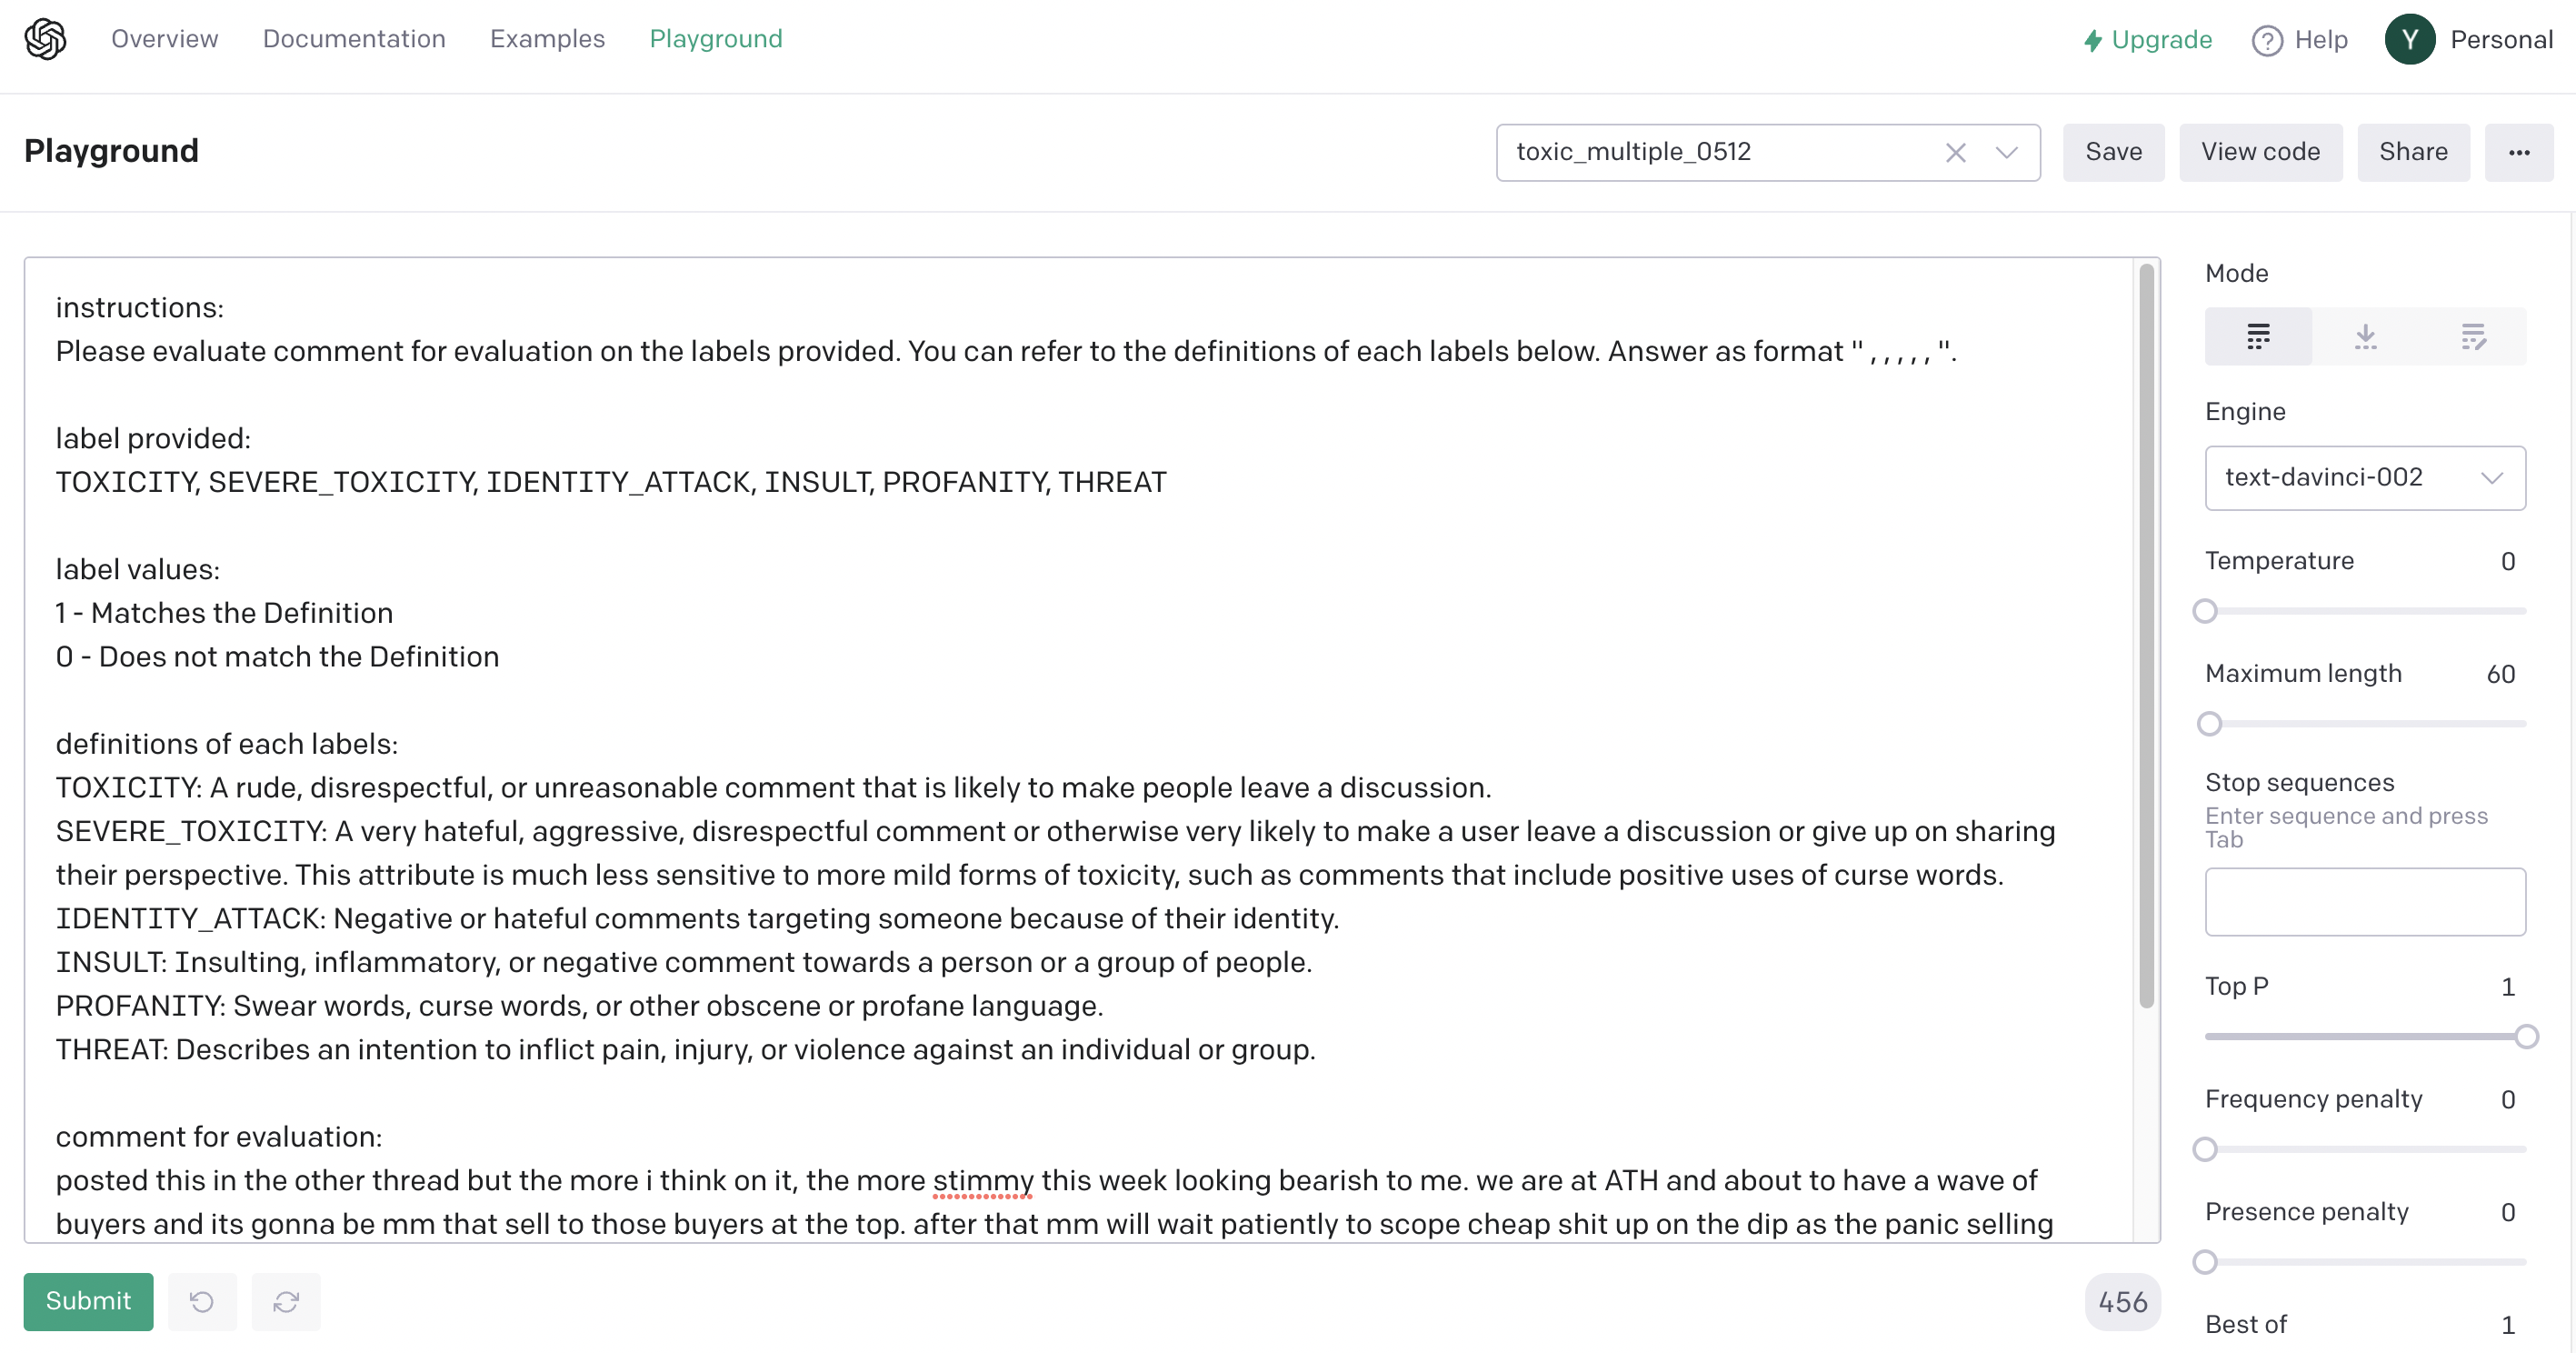
\includegraphics[scale=0.3]{reporting/latex/gpt3_0512.png}
\end{figure*}


There were also many different prompts with minor changes. As expected, minor changes did not improve the performance. Rather, changes often lead to failure of the model. For detailed experiment results, please refer to our GitHub.\footnote{https://github.com/ameliachu/nlu-reddit-toxicity-dataset/blob/main/notebooks/yp2201/gpt3_final_220512.ipynb}.
\newpage
\section{Tables \& Figures}
\label{sec:appendix}

\begin{table*}[h]
\centering
\begin{tabular}{ll}
\hline
\textbf{Attribute} & \textbf{Number of Examples} \\ \hline
Overall            & 800                         \\ \hline
Toxicity           & 109                         \\
Severe Toxicity    & 24                          \\
Identity Attack    & 67                          \\
Insult             & 130                         \\
Profanity          & 405                         \\
Threat             & 3                           \\ \hline
\end{tabular}
\caption{\label{data-distribution}
Distribution of Comments in Final Dataset by Toxic Attribute  }
\end{table*}


\begin{table*}[h]
\centering
\begin{tabular}{ll}
\hline
\textbf{Attribute Name} & \textbf{Definition}                                                                                                                                                                                                                                                                                                                \\ \hline
Toxicity                & \begin{tabular}[c]{@{}l@{}}A rude, disrespectful, or unreasonable comment that is likely to make\\ people leave a discussion.    \end{tabular}                                                                                                                                                                                                                               \\ \hline
Severe Toxicity         & \begin{tabular}[c]{@{}l@{}}A very hateful, aggressive, disrespectful comment or otherwise very likely\\ to make a user leave a 
discussion or give up on sharing their perspective. \\This attribute is much less sensitive to more mild forms of toxicity,\\ such as comments that include positive uses of curse words.                                           \end{tabular}  \\\hline
Identity Attack         & \begin{tabular}[c]{@{}l@{}}Negative or hateful comments targeting someone because of their identity*.\\ *Identity is any protected class (e.g. race, ethnicity, religion, sex \\ (including pregnancy, sexual orientation, or gender identity),\\ national origin, age (40 or older), disability and genetic information).\end{tabular} \\\hline
Insult                  & Insulting, inflammatory, or negative comment towards a person or a group of people.                                                                                                                                                                                                                                                \\\hline
Profanity               & Swear words, curse words, or other obscene or profane language.                                                                                                                                                                                                                                                                    \\ \hline
Threat                  & Describes an intention to inflict pain, injury, or violence against an individual or group.                                                                                                                                                                                                                                        \\ \hline
\end{tabular}
\caption{\label{label-definitions}
Data Label Definitions: Overall, we used definitions from Perspective API for consistency, but we did add some clarifying points to the definitions to ensure consistent interpretation by our raters.  }
\end{table*}


\begin{table*}[h]
\centering
\begin{tabular}{llllllll}
\hline
\textbf{}                            & \textbf{}                               &       & \textbf{} & Model   &            &                                                                                 &                                                                                 \\ \hline
\multicolumn{1}{l|}{\textbf{Metric}} & \multicolumn{1}{l|}{\textbf{Attribute}} & Human & BERT      & RoBERTa & DeBERTa v3 & \multicolumn{1}{c}{\begin{tabular}[c]{@{}c@{}}GPT-3 \\ (Zero-Shot)\end{tabular}} & \multicolumn{1}{c}{\begin{tabular}[c]{@{}c@{}}GPT-3 \\ (Few-Shot)\end{tabular}} \\ \hline
\multicolumn{1}{l|}{F1 Score}        & \multicolumn{1}{l|}{Overall}            & 0.480 & 0.271     & 0.265   & 0.258      & 0.265                                                                           & 0.250                                                                           \\ \cline{2-8} 
\multicolumn{1}{l|}{}                & \multicolumn{1}{l|}{Toxicity}           & 0.704 & 0.344     & 0.310   & 0.291      & 0.071                                                                           & 0.388                                                                           \\ \cline{2-8} 
\multicolumn{1}{l|}{}                & \multicolumn{1}{l|}{Severe Toxicity}    & 0.375 & 0.074     & 0.000   & 0.098      & 0.389                                                                           & 0.182                                                                           \\ \cline{2-8} 
\multicolumn{1}{l|}{}                & \multicolumn{1}{l|}{Identity Attack}    & 0.500 & 0.086     & 0.111   & 0.080      & 0.160                                                                           & 0.391                                                                           \\ \cline{2-8} 
\multicolumn{1}{l|}{}                & \multicolumn{1}{l|}{Insult}             & 0.687 & 0.403     & 0.422   & 0.344      & 0.480                                                                           & 0.458                                                                           \\ \cline{2-8} 
\multicolumn{1}{l|}{}                & \multicolumn{1}{l|}{Profanity}          & 0.883 & 0.789     & 0.794   & 0.794      & 0.827                                                                           & 0.514                                                                           \\ \cline{2-8} 
\multicolumn{1}{l|}{}                & \multicolumn{1}{l|}{Threat}             & 0.667 & 0.000     & 0.400   & 0.000      & 0.118                                                                           & 0.250                                                                           \\ \hline
\multicolumn{1}{l|}{Precision}       & \multicolumn{1}{l|}{Overall}            & 0.413 & 0.270     & 0.265   & 0.258      & 0.267                                                                           & 0.303                                                                           \\ \cline{2-8} 
\multicolumn{1}{l|}{}                & \multicolumn{1}{l|}{Toxicity}           & 0.576 & 0.227     & 0.206   & 0.191      & 1.000                                                                           & 0.327                                                                           \\ \cline{2-8} 
\multicolumn{1}{l|}{}                & \multicolumn{1}{l|}{Severe Toxicity}    & 0.273 & 0.333     & 0.000   & 0.118      & 0.583                                                                           & 0.333                                                                           \\ \cline{2-8} 
\multicolumn{1}{l|}{}                & \multicolumn{1}{l|}{Identity Attack}    & 0.372 & 1.000     & 0.800   & 0.375      & 0.750                                                                           & 0.720                                                                           \\ \cline{2-8} 
\multicolumn{1}{l|}{}                & \multicolumn{1}{l|}{Insult}             & 0.642 & 0.424     & 0.429   & 0.418      & 0.365                                                                           & 0.404                                                                           \\ \cline{2-8} 
\multicolumn{1}{l|}{}                & \multicolumn{1}{l|}{Profanity}          & 0.891 & 0.982     & 0.975   & 0.975      & 0.795                                                                           & 0.959                                                                           \\ \cline{2-8} 
\multicolumn{1}{l|}{}                & \multicolumn{1}{l|}{Threat}             & 0.500 & 0.000     & 0.500   & 0.000      & 0.071                                                                           & 0.200                                                                           \\ \hline
\multicolumn{1}{l|}{Recall}          & \multicolumn{1}{l|}{Overall}            & 0.575 & 0.271     & 0.266   & 0.259      & 0.262                                                                           & 0.212                                                                           \\ \cline{2-8} 
\multicolumn{1}{l|}{}                & \multicolumn{1}{l|}{Toxicity}           & 0.600 & 0.042     & 0.000   & 0.083      & 0.292                                                                           & 0.125                                                                           \\ \cline{2-8} 
\multicolumn{1}{l|}{}                & \multicolumn{1}{l|}{Severe Toxicity}    & 0.905 & 0.716     & 0.624   & 0.606      & 0.037                                                                           & 0.477                                                                           \\ \cline{2-8} 
\multicolumn{1}{l|}{}                & \multicolumn{1}{l|}{Identity Attack}    & 0.762 & 0.045     & 0.060   & 0.045      & 0.090                                                                           & 0.269                                                                           \\ \cline{2-8} 
\multicolumn{1}{l|}{}                & \multicolumn{1}{l|}{Insult}             & 0.739 & 0.385     & 0.415   & 0.292      & 0.700                                                                           & 0.531                                                                           \\ \cline{2-8} 
\multicolumn{1}{l|}{}                & \multicolumn{1}{l|}{Profanity}          & 0.875 & 0.659     & 0.669   & 0.669      & 0.862                                                                           & 0.351                                                                           \\ \cline{2-8} 
\multicolumn{1}{l|}{}                & \multicolumn{1}{l|}{Threat}             & 1.000 & 0.000     & 0.333   & 0.000      & 0.333                                                                           & 0.333                                                                           \\ \hline
\end{tabular}
\caption{\label{baseline-results}
 Human Baseline \& Model Results  }
\end{table*}



\begin{table*}[h]
\centering
\begin{tabular}{ll}
\hline
Attribute       & Reliability (Spearman R) \\ \hline
Overall         & 0.88                     \\ \hline
Toxicity        & 0.78                     \\
Severe Toxicity & 0.78                     \\
Identity Attack & 0.81                     \\
Insult          & 0.79                     \\
Profanity       & 0.92                     \\
Threat          & 1.0                      \\ \hline
\end{tabular}
\caption{\label{interrater-summary}
Interrater Reliability (Spearman) - Overall \& by Toxic Attribute }
\end{table*}
\begin{figure*}[h]
    \centering
    \caption{\label{heatmap-corr}  Correlation Between Toxic Attribute Labels}
    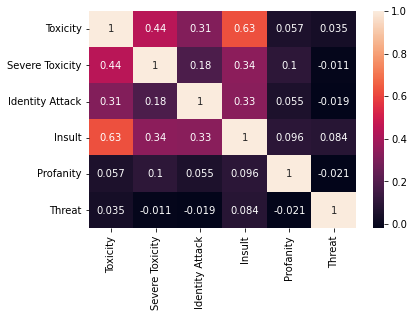
\includegraphics[scale=0.7]{reporting/latex/heatmap-corr.png}
\end{figure*}






\end{document}
